\section{Problem Introduction}
Pacman is a video game which utilizes textures of 8x8 pixels to render its core components as can be seen in Figure~\ref{PacmanLevelGrid}. 

\begin{figure}[H]
\centering
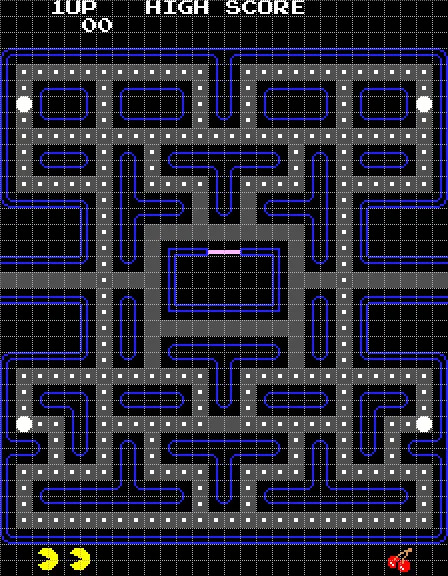
\includegraphics[width=0.4\linewidth]{Image-1.jpg}
\caption {Pacman level divided into squares of 8x8 pixels.\autocite{pittman_pac-man_2009}}\label{PacmanLevelGrid}
\end{figure}

Since the pixel length of a wall is 1 pixel, the wall textures all contain an asymmetry as seen in Figure~\ref{StraightWallTexture} and~\ref{CornerTexture}. The asymmetry is the basis of the visual appearance of levels which are formed by an oriented placing of these textures. 

\begin{figure}[H]
\centering

\includegraphics[width=0.4\linewidth]{Image-2.png}
\caption {A single wall square texture.\autocite{myself}}\label{StraightWallTexture}
\end{figure}

\begin{figure}[H]
\centering

\includegraphics[width=0.4\linewidth]{Image-3.png}
\caption {Square texture of corner.\autocite{myself}}\label{CornerTexture}
\end{figure}

Because of this asymmetry, it must be decided in what direction walls are clamped to ensure visual consistency. When all walls are clamped in the same direction we receive unsatisfactory results as seen on the left part of Figure~\ref{WallTextureAsymmetry}. 

\begin{figure}[H]
\centering

\includegraphics[width=0.4\linewidth]{Image-4.png}
\caption {Left - Incorrect orientation of tiles. Right - Correct orientation with walls clamped to appropriate direction. Walls on the left are clamped inward, to the right and walls on the right are clamped inwards to the left. The problem consists of determining which direction points "inwards"\autocite{myself}}\label{WallTextureAsymmetry}
\end{figure}

\begin{figure}[H]
\centering
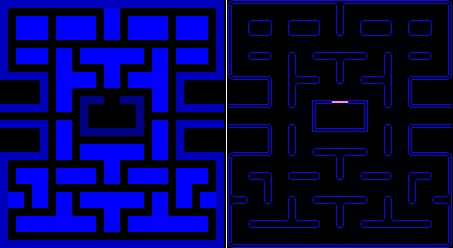
\includegraphics[width=0.8\linewidth]{Image-5.png}
\caption {The algorithm devised through this paper will convert from the image on the left to the one on the right, reconstructing the visual properties using a simplified outline.\autocite{myself}}\label{LevelWallConversion}
\end{figure}

This problem will be reduced to elements of graph theory.